\documentclass[10pt,a4paper]{article}
\usepackage[latin1]{inputenc}
\usepackage{amsmath}
\usepackage{amsfonts}
\usepackage{amssymb}
\usepackage{color}
\usepackage{graphicx}
\usepackage{hyperref}
\usepackage{enumitem}
\usepackage{graphicx}
\hypersetup{
	colorlinks=true,
	linkcolor=blue,
	filecolor=magenta,
	urlcolor=cyan,
}
\RequirePackage[left=01.1cm,top=3cm,right=1.5cm,bottom=2.5cm,nohead,nofoot]{geometry}

\author{\vspace{0.4cm}
	Anirudh N J \\\vspace{0.4cm}
	Somesh Devagekar \\\vspace{0.8cm}
	Raina Thomas}

\title{
	\vspace*{5cm}
	\textbf{Scientific Experimentation and Evaluation}
	}
	
\date{\color{blue}April 10, 2019}			
\begin{document}
	
\begin{titlepage}

	\maketitle
	
\end{titlepage}

\Large\textbf{\color{blue}LEGO NXT Project Implementation}

\Large
\begin{enumerate}[label=\Roman*]

\item
\vspace{0.5cm}
\Large{\textbf{Aim}}\\

The aim of this project is to construct a LEGO NXT differential drive robot and measure the observable end pose variation for three different trajectories: an arc to the left, driving straight and an arc to the right.
\vspace{0.5cm}

The experiment of measuring the end pose was done by measuring the pose using markers and Computer Vision.
   

\vspace{0.5cm}
\item
\Large{\textbf{Experimental Setup}}\\
\vspace{0.5cm}

To reproduce the above experiment the following equipment are needed :
\begin{enumerate}
    \item
    White A1 Sheet
    \item
    Camera - Microsoft 
    \item
    Assembled robot - Lego NXT 
    \item
    Scales for measuring the length 
    \item
    Vision markers
\end{enumerate}
\vspace{0.5cm}

The general steps to setup the experiment are as following :
\begin{enumerate}
    \item
    Place the White A1 sheet on a flat surface.  Try to remove any bends in the sheet and keep the paper as flat as possible. This will be called the 'map' on which the robot will move on. The measurement system is made of the robot, pen, scale and a paper. 
    \item
    Mark the center of the A1 sheet using the scale and a pencil.
    \item
    Draw the template drawing of the "floor space" taken by the robot as shown in the figure. Concept of "Behavior-shaping constraint" is used to prevent wrong initial placement of the robot.
    
    
    \begin{figure}[h]
	\centering
    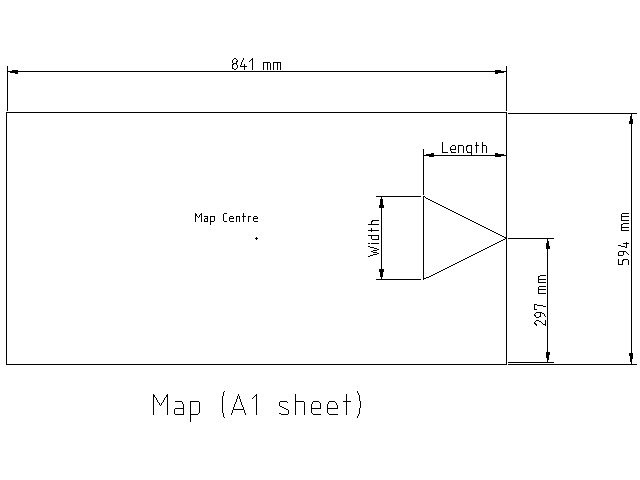
\includegraphics[width=0.6\linewidth ]{Template.png}
    \caption{ Template drawing of the Map along with dimensions}
    \end{figure}

    \item
    Assemble the robot using the manual given with the LEGO NXT box. Install the OS to the controller of the robot. The Lego robot is the device under test(DUT). 
    \item
    We assume that the driving axle is towards the front(leading edge) of the robot and that the robot origin lies in the centre of the driving axle.
    \item
    Place the robot on the A1 sheet over the marked template.
    \item
	The measurands are the distance between the initial and end positions and the angles between the center of the robot and the tail of the robot.
    
\end{enumerate}
\vspace{0.5cm}

The reference images of the DUT and the proposed marker tracking visualization are given below.

\begin{figure}[h]
	\centering
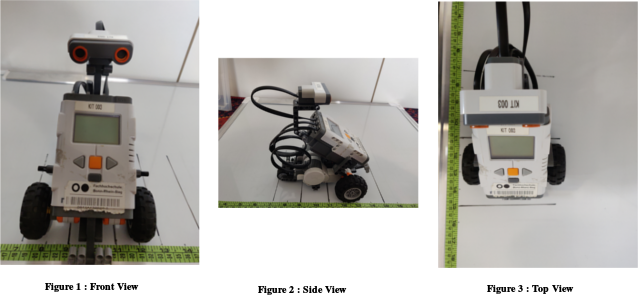
\includegraphics[width=0.8\linewidth ]{pose.png}
\caption{ Views of the DUT- with approximate dimensions}
\end{figure}

\vspace{0.5cm}
\newpage
\item
\Large{\textbf{Procedure}}\\

\begin{enumerate}
	\item
	For this experiment the camera should be placed rigidly directly above the experiment setup such that the full map is visible in the camera frame. 
	\item
	Before beginning the experiment the camera should be calibrated and the obtained parameters should be used to compensate for the lens distortion and other errors in the image. 
	\item
	Two small markers should be attached on the flat surface of the robot, one on the front and one on the rear of the robot. The markers should be visible in the camera frame captured by the overhead camera. (The two markers should have different ID to distinguish between them)
	\item
    Using Computer-vision the two markers on the robot can be tracked and localized. The centre of the markers can be found and be used to calculate the offset from the actual robot origin using a scale or any other measuring device.
	\item
	The robot is programmed to move using the initial pose and the desired final pose.
	\item
	The initial pose and the final pose can be found by CV and position and pose in the required form can be extracted.
	\item
	20 measurements would be performed for each trajectory. Mean and standard deviation will be computed from the measurement. These measured values would be used to compute the accuracy and precision of the pose variation. 
\end{enumerate}
\vspace{0.5cm}

\begin{figure}[h]
	\centering

\includegraphics[width=0.2\linewidth ]{marker.png}
\caption{ Example Aruco marker for computer vision}
\end{figure}


\item
\textbf{Observations}\\
\begin{enumerate}
	\item
	This experiment accuracy and precision depends highly on the setting up of the camera and the markers correctly.
	\item
	Since the experiment does not rely on any manual intervention or has no moving parts like the pen, the precision is very high.
\end{enumerate}
\vspace{0.5cm}

\item
\textbf{Conclusion}\\

\item
\textbf{Result}\\

\end{enumerate}






\end{document}


